% DocuFlow Class v1.0 (Snippets)
% Created by Lucas Schmirl, 2025.

\section{Allgemeine \LaTeX Beispiele}

Querverweise werden in \LaTeX{} automatisch erzeugt und verwaltet, damit sie leicht aktualisiert werden können.
Beispiele sind~\cite{Ko05a},~\cite{Ko05b},~\cite{MiGo05},~\cite{TeGo14},~\cite{HuHa07}.
Es wird dringend empfohlen, Biber oder BibTeX zu verwenden (wie in diesen Beispielen).
Die Quellen werden in \verb|bibliography.bib| definiert, (Templates verfügbar).\\

Abkürzungen wie die folgenden sind im Abkürzungsverzeichnis vermerkt:
\ac{CPU}, \ac{RAM}, und \ac{GPU}. Diese können nach der Definition in \texttt{acronym} in \texttt{main.tex} verwendet werden.\\

Eine \glqq{}schöne\grqq{} Farbe ist \textcolor{FAVgreen}{dieses Grün (RGB:~177,179,48)}.\\

\noindent Wenn ein neuer Absatz \textcolor{red}{nicht} eingerückt werden soll funktioniert das so.\\

Anführungszeichen können auf \glq{}diese\grq{}, 'diese' und \glqq{}jene\grqq{} Weise verwendet werden.\\

So macht man einen Zeilenumbruch.\\
Und so einen Seitenumbruch.\clearpage

    
    \subsection{Abbildungen}

        \begin{figure}[!htbp]
            \centering
            \includegraphics[width=0.5\linewidth]{PICs/hund.png}
            \caption{Das ist ein Hund.}
            \label{Abb:hund}
        \end{figure}

        Für das Einfügen von Bildern kann auch das \verb|figure-macro| der Klasse verwendet werden.
        
        \DFfigure[0.5\linewidth, angle=-90]{PICs/hund}{Der selbe Hund (rotiert).}{fig:smallFigure}


    \clearpage
    \subsection{Tabellen}

        \begin{table}[!htbp]
                \centering
                \begin{tabular}{| p{0.3\linewidth} | p{0.3\linewidth} | p{0.3\linewidth} |}\hline
                %\begin{tabular}{| c | l | r |}\hline
                Datum & Produktionsschritt & Abteilung\\\hline
                15.02.2025 & Rohstoffmischung & Chemielabor\\
                17.02.2025 & Qualitätsprüfung & Labor\\
                20.02.2025 & Abfüllung & Produktion\\
                22.02.2025 & Verpackung & Logistik\\\hline
                \end{tabular}
                \caption{Produktionsplan für Reinigungsmittel \glqq{}EcoClean\grqq{}.}\label{tab:1}
            \end{table}


    \subsection{Verweise, Links}
        Das ist ein Verweis auf Tabelle~\ref{tab:1}. Das gezeigte Tabellenformat ist nur ein Beispiel.
        Tabellen können individuell gestaltet werden, dazu gerne auch mal dieses \hyperref{https://www.tablesgenerator.com/}{category}{name}{Tool} austesten.\\

        Hier wird zum Beispiel auf Abbildung~\ref{Abb:hund} verwiesen.\\


    \subsection{Mathematische Formeln}
    Im nächsten Unterkapitel werden Formeln wie z.B. Formel~\ref{Gl:1} dargestellt.
    Griechische Buschtaben können auf diese weise eingefügt werden: 
    $\alpha, \beta, \gamma, \rho, \sigma, \delta, \epsilon$.

        \begin{align}
            x &= -\frac{p}{2}\pm\sqrt{\frac{p^2}{4}-q}\label{Gl:1}\\
            e^{i \pi} + 1 &= 0\label{Gl:2}\\
            C &= \sum_{n=-\infty}^{+\infty} f(\frac{\partial x}{\partial y}w)
        \end{align}


    \clearpage
    \subsection{Code}

    Code kann mithilfe des Pakets \verb|listing| dargestellt werden.
        \begin{lstlisting}[language=C++,name={C++ Beispiel},label={sc:bsp:1}]
            #include <iostream>

            void SayHello(void)
            {
                // Kommentar
                cout << "Hello World!" << endl;
            }

            int main(int argc, char **argv)
            {
                SayHello();
                return 0;
            }
            \end{lstlisting}

    \subsection{Grafiken (Zeichnen)}
    % This is how to draw manually
    \begin{figure}[!htbp]
        \centering
        \begin{tikzpicture}
            \node[draw=orange, fill=orange!20] (a) {\large A};
            \node[draw=yellow, fill=yellow!20, right= of a] (b) {\Large B};
            \node[circle, draw=green, fill=green!20, right= of b] (c) {\Large C};
            \draw[->] (a) -- (b);
            \draw[->>] (b) -- (c);
        \end{tikzpicture}\caption{Selbst gezeichnete Grafik: \hyperref{https://greysonwesley.com/files/TikZCheatsheet.pdf}{}{}{Cheatsheet}}\label{fig:my_graph}
    \end{figure}
    
    % This is how to draw manually (by Gii)
    \begin{figure}[!htbp]
        \centering
        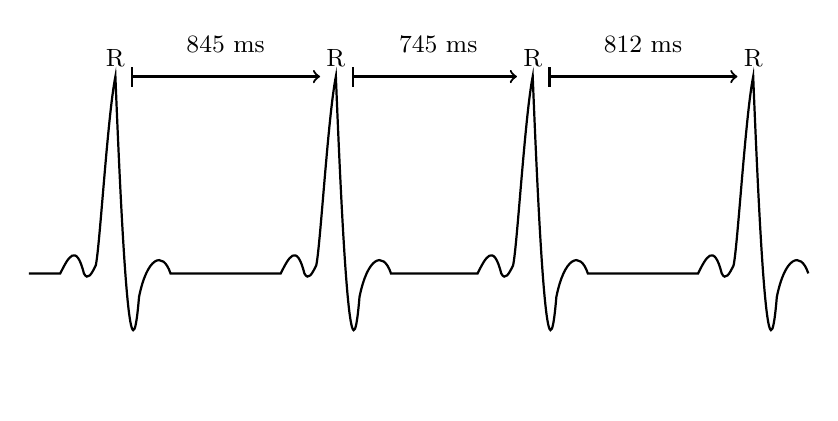
\begin{tikzpicture}[scale=1, every node/.style={font=\small}]
            % EKG-Tracing mit variierenden Abständen
            \draw[thick]
            (0,0) -- (0.4,0)
            .. controls (0.5,0.2) and (0.6,0.4) .. (0.7,0)
            .. controls (0.75,-0.1) and (0.8,0) .. (0.85,0.1)
            .. controls (0.9,0.3) and (1,2) .. (1.1,2.5)
            .. controls (1.2,0) and (1.3,-1.5) .. (1.4,-0.3)
            .. controls (1.5,0.2) and (1.7,0.3) .. (1.8,0)
            -- (3.2,0)
            .. controls (3.3,0.2) and (3.4,0.4) .. (3.5,0)
            .. controls (3.55,-0.1) and (3.6,0) .. (3.65,0.1)
            .. controls (3.7,0.3) and (3.8,2) .. (3.9,2.5)
            .. controls (4.0,0) and (4.1,-1.5) .. (4.2,-0.3)
            .. controls (4.3,0.2) and (4.5,0.3) .. (4.6,0)
            -- (5.7,0)
            .. controls (5.8,0.2) and (5.9,0.4) .. (6.0,0)
            .. controls (6.05,-0.1) and (6.1,0) .. (6.15,0.1)
            .. controls (6.2,0.3) and (6.3,2) .. (6.4,2.5)
            .. controls (6.5,0) and (6.6,-1.5) .. (6.7,-0.3)
            .. controls (6.8,0.2) and (7.0,0.3) .. (7.1,0)
            -- (8.5,0)
            .. controls (8.6,0.2) and (8.7,0.4) .. (8.8,0)
            .. controls (8.85,-0.1) and (8.9,0) .. (8.95,0.1)
            .. controls (9.0,0.3) and (9.1,2) .. (9.2,2.5)
            .. controls (9.3,0) and (9.4,-1.5) .. (9.5,-0.3)
            .. controls (9.6,0.2) and (9.8,0.3) .. (9.9,0);
            
            % R-Markierungen bei Peaks
            \node[above] at (1.1,2.5) {R};
            \node[above] at (3.9,2.5) {R};
            \node[above] at (6.4,2.5) {R};
            \node[above] at (9.2,2.5) {R};
            
            % Pfeile, horizontal auf Höhe der R, Start/Ende weiter entfernt
            \draw[|->, thick] (1.3,2.5) -- (3.7,2.5);
            \node[above=5pt] at (2.5,2.5) {845 ms};
            
            \draw[|->, thick] (4.1,2.5) -- (6.2,2.5);
            \node[above=5pt] at (5.2,2.5) {745 ms};
            
            \draw[|->, thick] (6.6,2.5) -- (9.0,2.5);
            \node[above=5pt] at (7.8,2.5) {812 ms};
        \end{tikzpicture}
        \caption{Schematische Darstellung eines EKG-Signals mit RR-Intervallen.}
        \label{fig:puls}
	\end{figure}

    % This file was created with a plot in python using tikzmaker (https://tikzmaker.com/editor)
    \begin{figure}[!ht]
        \centering
        \resizebox{0.7\textwidth}{!}{
        \begin{circuitikz}
        \tikzstyle{every node}=[font=\LARGE]
            \draw (7.5,13.25) to[american voltage source,l={ \small 5V 100mA}] (9.5,13.25);
            \draw (9.5,13.25) to[rmeter, t=V,l={ \small 3.4V}] (13.5,13.25);
            \draw [ fill={rgb,255:red,197; green,255; blue,71} ](13.5,13.25) to[lamp] (13.5,11.5);
            \draw (7.5,11.5) to[R,l={ \small 1k$\Omega$}] (10.75,11.5);
            \draw [short] (7.5,13.25) -- (7.5,11.5);
            \draw [short] (10.75,11.5) .. controls (12.25,11.5) and (12.25,11.5) .. (13.5,11.5);
        \end{circuitikz}}\caption{Erstellt mithilfe von \hyperref{https://tikzmaker.com/editor}{category}{name}{tikzmaker}.}\label{fig:tikzmaker}
    \end{figure}
    
    % This file was created with a plot in python using tikzplotlib v0.10.1. (https://pypi.org/project/tikzplotlib/)
    \begin{figure}\centering
        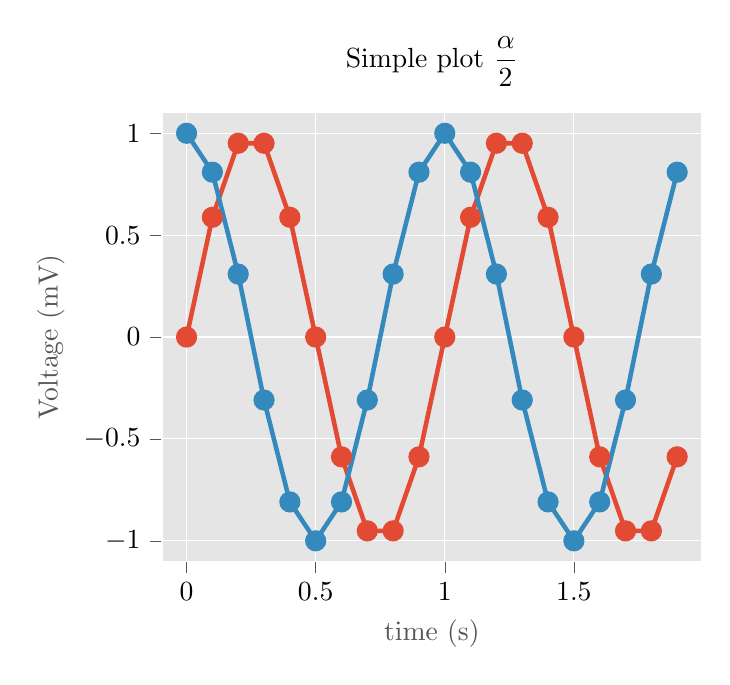
\begin{tikzpicture}
            \definecolor{chocolate2267451}{RGB}{226,74,51}
            \definecolor{dimgray85}{RGB}{85,85,85}
            \definecolor{gainsboro229}{RGB}{229,229,229}
            \definecolor{steelblue52138189}{RGB}{52,138,189}
            \begin{axis}[
                axis background/.style={fill=gainsboro229},
                axis line style={white},
                tick align=outside,
                tick pos=left,
                title={Simple plot \(\displaystyle \frac{\alpha}{2}\)},
                x grid style={white},
                xlabel=\textcolor{dimgray85}{time (s)},
                xmajorgrids,
                xmin=-0.095, xmax=1.995,
                xtick style={color=dimgray85},
                y grid style={white},
                ylabel=\textcolor{dimgray85}{Voltage (mV)},
                ymajorgrids,
                ymin=-1.1, ymax=1.1,
                ytick style={color=dimgray85}
                ]
                \addplot [line width=1.64pt, chocolate2267451, mark=*, mark size=3, mark options={solid}]
                table {%
                0 0
                0.1 0.587785252292473
                0.2 0.951056516295154
                0.3 0.951056516295154
                0.4 0.587785252292473
                0.5 1.22464679914735e-16
                0.6 -0.587785252292473
                0.7 -0.951056516295154
                0.8 -0.951056516295154
                0.9 -0.587785252292473
                1 -2.44929359829471e-16
                1.1 0.587785252292474
                1.2 0.951056516295154
                1.3 0.951056516295154
                1.4 0.587785252292473
                1.5 3.67394039744206e-16
                1.6 -0.587785252292473
                1.7 -0.951056516295154
                1.8 -0.951056516295154
                1.9 -0.587785252292473
                };
                \addplot [line width=1.64pt, steelblue52138189, mark=*, mark size=3, mark options={solid}]
                table {%
                0 1
                0.1 0.809016994374947
                0.2 0.309016994374947
                0.3 -0.309016994374948
                0.4 -0.809016994374947
                0.5 -1
                0.6 -0.809016994374947
                0.7 -0.309016994374948
                0.8 0.309016994374947
                0.9 0.809016994374947
                1 1
                1.1 0.809016994374947
                1.2 0.309016994374947
                1.3 -0.309016994374947
                1.4 -0.809016994374947
                1.5 -1
                1.6 -0.809016994374948
                1.7 -0.309016994374946
                1.8 0.309016994374947
                1.9 0.809016994374947
                };
            \end{axis}
        \end{tikzpicture}\caption{Erstellt mithilfe von \hyperref{https://pypi.org/project/tikzplotlib/}{category}{name}{Python tikzplotlib}.}\label{fig:tikzplotlib}
    \end{figure}
    \clearpage